\section{Discrete Wavelet Transform}

\subsection{One dimensional DWT}

\begin{figure}
    \centering
    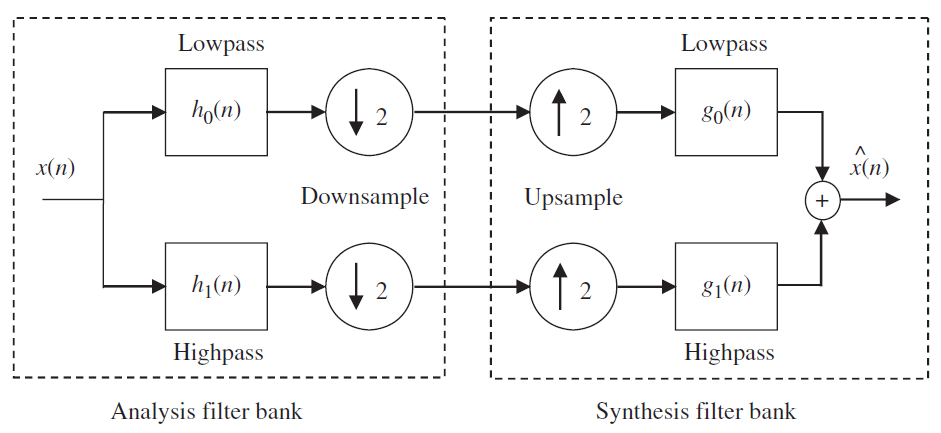
\includegraphics[scale=0.5]{dwt_1d_anal_synth.png}
    \caption{1-D DWT, two-band wavelet analysis and synthesis filter banks \cite{jpeg_suite}}
    \label{fig:dwt_1d_anal_synth}
\end{figure}

The linear convolution (filtering) of sequences $x(n)$ and $h(n)$ is defined as in equation \ref{eq:convolution}:
\begin{equation}
    y(n)=\sum_{m=-\infty}^{\infty}x(m)h(n-m)
\label{eq:convolution}
\end{equation}
The one dimensional discrete wavelet transform can be depicted as successive applications (convolutions) of
one seleceted pair of high and low-pass filters. The output of such application is then followed
by downsampling by the factor of two. For example, it can be achieved by discarding samples with
odd indices after each of filtering operation. It is better visualized in the Figure \ref{fig:dwt_1d_anal_synth}. \cite{jpeg_suite} 
The pair of low and high-pass filters is known as analysis filter bank in the encoding process.
In the signal decoding process it is featured as a synthesis filter bank. The decoding step requires
using the inverse of discrete wavelet transform. 

The idea of using lowpass filter is the preservation of low frequencies of a signal while trying
to eliminate or at least attenuate the high frequencies. In a result the output signal is the blurred
version of the original one. Therefore, the operating principle of the highpass filter is completely
opposite. As a result of applying such filter, the high frequencies of the signal are preserved and
the low ones are discarded or at least dimnished. The output is a signal consisting of edges, textures
and other details. \cite{jpeg_suite} 

Take into consideration a one dimensional signal $x(n) = \{55, 234, 70, 21, 88, 37\}$. It can be better
understood as values of pixels in a part of the grayscale image row. It is followed with a pair of low
and highpass filters designated by $h_{0}(n)$ and $h_{1}(n)$ respectively. An example of such pair is
a lowpass filter $h_{0}(n) = \{-1, 2, 6, 2, -1\}/8$ and a highpass filter $h_{1}(n) = \{-1, 2, -1\}/2$. They are both
symmetric and consist of only integer taps. Such pair can be presented in the notaion of (5, 3) filter bank.
This convension indicates that the length of lowpass filter is five and the length of highpass filter is three.
In fact the analysis fitler bank presented here was firstly proposed by LeGall and Tabatabai in 1988 and
is used in the JPEG 2000 standard for lossless compression of images. The filtering operation has to
be defined at the signal boundaries. Therefore, the one dimensional signal is extended in both directions.
The Part 1 of the JPEG 2000 standard requires symmetrical extension to be perfomed in such case. \cite{jpeg_suite}
After applying the required symmetrical padding the signal is extended to
$x(n) = \{21, 70, 234, 55, 55, 234, 70, 21, 88, 37, 37, 88, 21, 70\}$. Then, the lowpass fitler is applied
resulting in $x'_{0}(n) = \{197.25, 75.5, 98.375, 67.125, 45.375\}$ and the higpass one which results in
$x'_{1}(n) = \{44.75, -85.75, 29, 12.75, -29.5\}$.

\begin{figure}
    \centering
    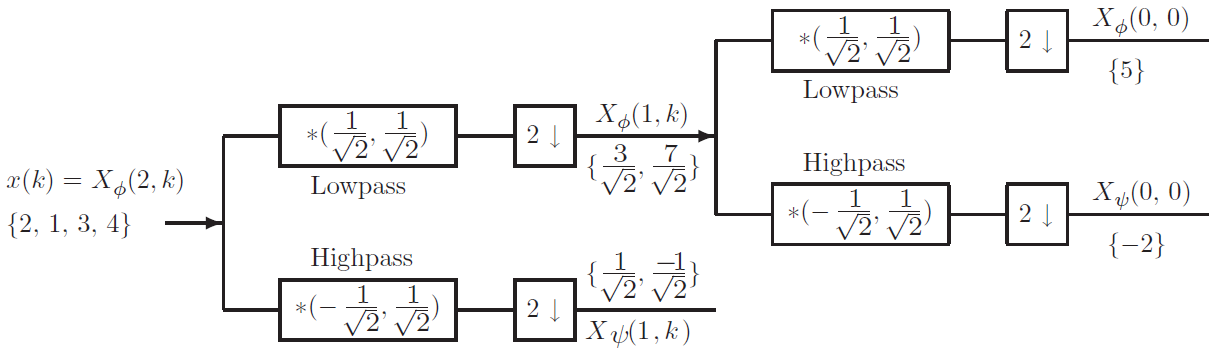
\includegraphics[scale=0.45]{dwt_1d_2_level.png}
    \caption{Computation of a 2-level 4-point DWT using a two-stage two-channel Haar analysis filter bank \cite{dwt_impl}}
    \label{fig:dwt_1d_2_level}
\end{figure}

The next example shows how to compute the two levels of discrete wavelet transform. To speed up the process
no padding option is chosen this time which makes it non-compliant with the JPEG 2000 standard.
The filter used here is the most basic one, i.e. Haar analysis filter bank. It is the first wavelet
from the Daubechies wavelet family. The calculation process is visualized in the Figure \ref{fig:dwt_1d_2_level}. \cite{dwt_impl}

The input is chosen as 4-point signal $X_{\phi}(2, k) = \{2, 1, 3, 4\}$. This notaion emphasizes the fact
that it is approximation of the input at scale 2. The so called scalling coefficients (or in other term
approximation at scale 1) $X_{\phi}(1, k)$ are computed by convolving the input $x(k)$ with the low-pass
Haar filter impulse response $l(k) = \{1/\sqrt{2}, 1/\sqrt{2}\}$. In the next step there is downsampling
by a factor of 2 applied. The output of convolution has five values. The middle three from these fives 
correspond to cases where both the given input values overlap with the impuse response. As it was described
earlier, the odd values are preserved in the downsampling process. In a result first and third value of these
three middle ones are the approximation output $X_{\phi}(1, k)$. In the similar way, the detail coefficients
at scale 1 $X_{\psi}(1, k)$ are computed. The input $x(k)$ is convoled with the high-pass filter impulse
response $h(k) = \{-1/\sqrt{2}, 1/\sqrt{2}\}$. Then the downsampling by factor of 2 is perfomed.
Note that only only approximation output $X_{\phi}(1, k)$ of the first stage goes to the second one.
The $X_{\phi}(0, 0)$ and $X_{\psi}(0, 0)$ are calculated accordingly at the end of the second stage. \cite{dwt_impl}

\subsection{Two dimensional DWT}

\begin{figure}
    \centering
    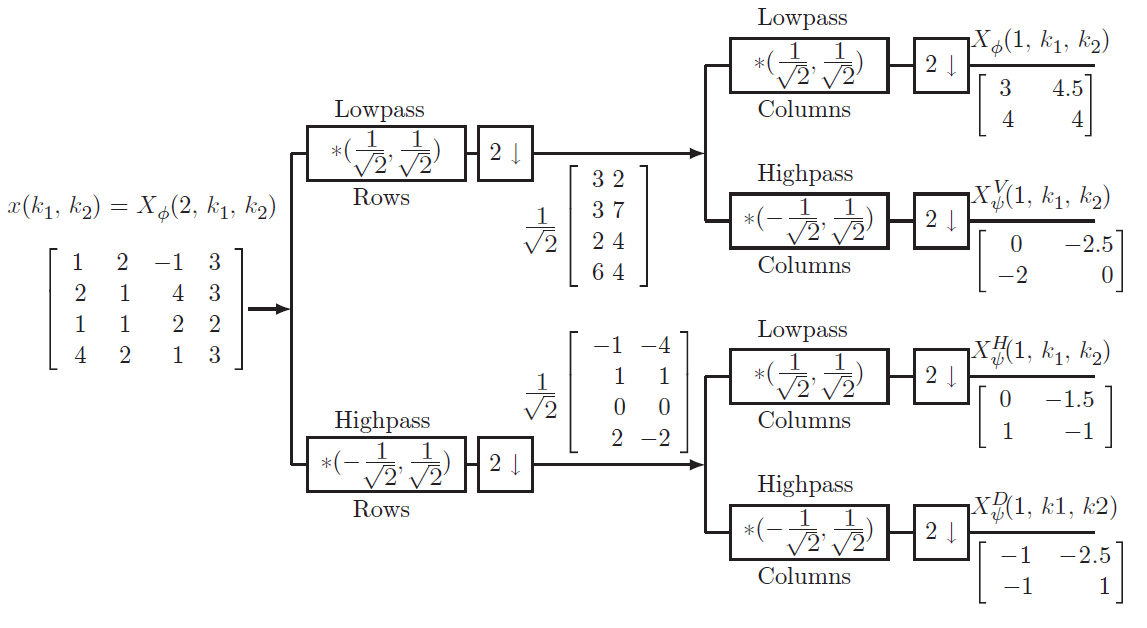
\includegraphics[scale=0.45]{dwt_2d_1_level.png}
    \caption{Computation of a 1-level 4 $\times$ 4 2-D Haar DWT using a two-stage filter bank \cite{dwt_impl}}
    \label{fig:dwt_2d_1_level}
\end{figure}

Something something\dots Figure \ref{fig:dwt_2d_1_level} \cite{dwt_impl}

% Something about DWT -> some specific info, new section probably to each of them
\begin{figure}
    \centering
    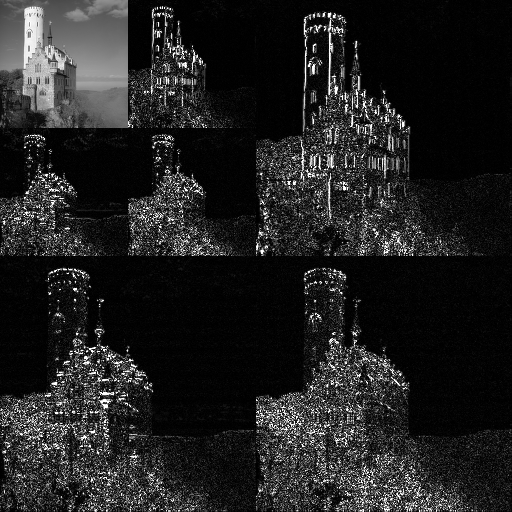
\includegraphics[scale=0.7]{dwt_2d_example_wiki.png}
    \caption{2D DWT applied 2 times to an exemplary image \cite{dwt_example_wiki}}
    \label{fig:dwt_2d_example_wiki}
\end{figure}

An example of the 2D discrete wavelet transform that is used in JPEG2000 \ref{fig:dwt_2d_example_wiki}.
The original image is high-pass filtered, yielding the three large images, each describing local changes
in brightness (details) in the original image. It is then low-pass filtered and downscaled, yielding
an approximation image; this image is high-pass filtered to produce the three smaller detail images and low-pass
filtered to produce the final approximation image in the upper-left. \cite{dwt_example_wiki}

\subsection{DWT main features}

\begin{itemize}
    \item The DWT is essentially a set of bandpass filters. However, it is efficiently implemented
    using a set of lowpass and highpass filters recursively.
    \item The computational complexity of computing the DWT is O(N).
    \item There are basically two approaches to implement the DWT efficiently. The first approach is
    to evaluate the required convolutions using the polyphase filter structure. Transform methods
    are not used to carry out the convolution, as the length of the impulse response of the
    filters is short.
    \item The other approach is to factorize the polyphase matrix into a product of a set of sparse
    matrices.
    \item The 2-D DWT, with separable filters, is usually computed by the row-column method. That
    is, 1-D DWT of all the columns is computed, and then the 1-D DWT of all the resulting
    rows is computed. The order of the computation can also be reversed.
    \item In the implementation of the DWT, additional memory of about half the size of the data is
    required. For an in-place computation, data reordering is required.
    \item In implementing the asymmetric filters, data expansion problem occurs due to the finite
    length of the data.
    \item Symmetric filters provide linear phase response and an effective solution to the border
    problem.
\end{itemize}

\section{Part 2 of the JPEG 2000}

% Part2 in details
% write down different filters and basic ones

\subsection{Introduction}

As JPEG 2000 developed, many ideas for value-added capabilities emerged. It was not
feasible to include them in the Part 1 Core (ISO/IEC, 2004a) – originally published
in 2000 – so additional parts were created. The Part 2 standard, published as ISO/IEC
15444-2 or ITU Recommendation T.801 (ISO/IEC, 2004b), contains multiple extensions
of JPEG 2000 that were not large enough to merit entire documents of their own.
Unlike the JPEG 2000 Part 1 Core, where decoders are expected to handle all the
code-stream functionality, Part 2 is a collection of options that may be implemented `a la
carte to meet specific market requirements. Moreover, sections within an extension annex
can be implemented separately (e.g. subsets of the extended file format JPX). Hence,
some extension features may appear across a wide spectrum of JPEG 2000 applications,
while others will be less common in decoders.
The extensions in Part 2 cover a disparate set of topics that modify or add to the Part 1
JPEG 2000 processing chain. Some tools improve the compression efficiency and/or visual
appearance of compressed images, while others modify or extend the functionality in other
ways. To set the stage for the remainder of this chapter, we list the major topics with a
pointer to their location within the Part 2 standard:

Compression efficiency
\begin{itemize}
    \item Variable DC offset (VDCO) - Annex B
    \item Variable scalar quantization (VSQ) - Annex C
    \item Trellis coded quantization (TCQ) - Annex D
    \item Extended visual masking - Annex E
    \item Arbitrary wavelet decomposition - Annex F
    \item Arbitrary wavelet transform kernel - Annexes G and H
    \item Multiple component transform - Annex J
    \item Nonlinear point transform - Annex K
\end{itemize}

Functionality
\begin{itemize} 
    \item Geometric manipulation - Annex I
    \item Single-sample overlap (SSO/TSSO) - Annex I
    \item Precinct-dependent quantization - Amendment 1
    \item Extended region of interest - Annex L
    \item Extended file format/metadata (JPX) - Annexes M and N
    \item Extended capabilities signaling - Amendment 2
\end{itemize}

\subsection{Arbitrary Decomposition}

JPEG 2000 Part 1 allows only one wavelet decomposition structure: the well-known
Mallat dyadic decomposition. Although this decomposition represents a good first choice
across a broad spectrum of imagery, other decomposition styles can improve the image
quality over specialized image classes and allow unequal size reductions in the horizontal
and vertical dimensions of reduced resolution extracts.
Other decomposition styles described with some regularity in the wavelet literature
include the full packet tree and its derivatives. The packet decomposition derivatives can
outperform the dyadic decomposition at maintaining regular fine-grain texture and work
well on synthetic aperture radar imagery. The US Federal Bureau of Investigation uses
a 500 ppi fingerprint compression standard, WSQ (CJIS, 1997), with a decomposition
specialized for the characteristics of fingerprint imagery at 500 dpi. Figure 2.7 shows
some of these decompositions.
In addition to prespecified decomposition structures, wavelet packet analysis can be
used to design custom decompositions for specific images or image types (Coifman and
Wickerhauser, 1992; Ramchandan anad Vetterli, 1993; Meyer, Averbuch, and Stromberg,
2000). Such approaches start with a large decomposition tree and locate a good decomposition
based upon a chosen optimization metric.

\subsection{Arbitrary Wavelet Transforms}

JPEG 2000 Part 1 includes only two wavelet transforms: the irreversible 9-7I and the
reversible 5-3R, both specified with periodic symmetric preextension of the signal at
the boundaries. While these filters work well for compressing a wide range of image
types, certain image classes compress better with other wavelets. To allow this flexibility,
Part 2 broadens the range of wavelet transforms that can be used to include not only the
wider range of whole-sample symmetric (WS) filters, but also half-sample symmetric (HS)
filters and generic nonsymmetric filters. This ability to handle generic filters makes JPEG
2000 powerful not only for niche compression applications but also as a research tool. \cite{jpeg_suite}


\section{Computer architecture}

% some architectural blah blah, multiscaral, exhausted processor speed up curve -> cores, cores, more cores
    

\section{Known solutions}

% I'd go only with supervisor's papers and Kakadu, probably one section, several paragraphs

\begin{itemize}
    \item state of the art, literature research (all sources in the thesis have to be referenced)
    \item description of known solutions, algorithms
\end{itemize}
